\section{Detection Efficiency of the XENON100 PMTs}
\label{secQE}

The spectral response of a PMT can be characterized by the radiant sensitivity or with a QE of the photocathode. 
Radiant sensitivity is the photoelectric current from the photocathode normalized to the incident flux at a given wavelength. QE is the ratio of photoelectrons emitted from the photocathode and the number of incident photons.

Radiant sensitivity and QE efficiency are usually measured using a precisely calibrated light sensor as a reference, which can be either a standard phototube or a semiconductor detector. First, the incident radiant flux {\it L} [W] of the light source is measured with this device. Then, the photocurrent {\it I} [A] is measured for the PMT. The radiant sensitivity SK of the phototube is calculated as:
\begin{equation}
\mathrm{SK} = \frac{I}{L}\ \mathrm{[A/W]}
\end{equation}
 
The QE is obtained from the measured radiant sensitivity~\cite{HamamatsuHandbook}:
\begin{equation}
\mathrm{QE} = \frac{h c}{\lambda e}\cdot \mathrm{SK}\cdot \text{100\%},
\end{equation}
where $\lambda$ is the wavelength of the incident light in [nm], $h$ is Planck's constant, $c$ is  the velocity of light in vacuum, $e$ is electron charge.

\begin{figure}[!b]
\centering
\subfigure[]{
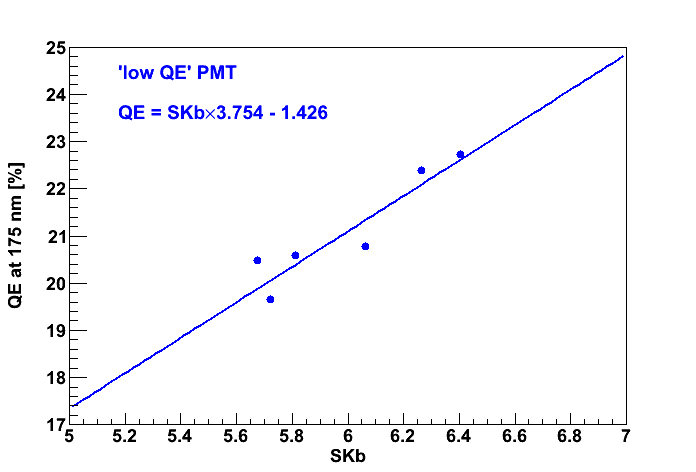
\includegraphics[width=0.475\linewidth]{plots/QE/plotQEvsSKb_lowQE.png}
\label{figSKBvsQE_1}}
\subfigure[]{
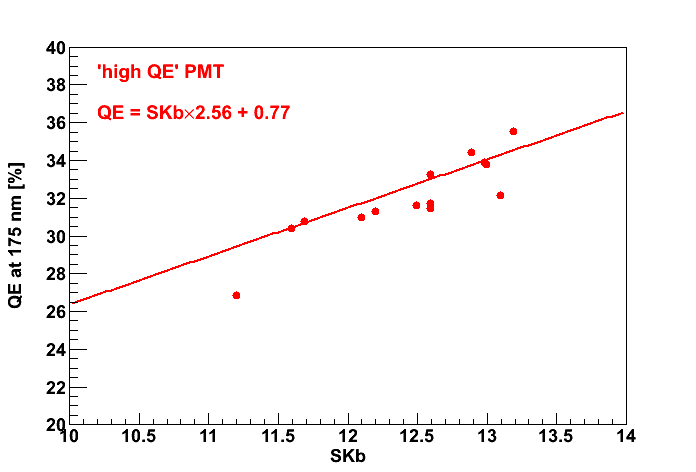
\includegraphics[width=0.475\linewidth]{plots/QE/plotQEvsSKb_highQE.png}
\label{figSKBvsQE_2}}
\caption[Correlation between sensitivity of the cathode to blue light (SKb) and quantum efficiency (QE) for the XENON100 PMTs]{Correlation between sensitivity of the cathode to blue light (SKb) and quantum efficiency (QE) for the low QE (a)  and high QE (b) XENON100 PMTs \cite{PMTmassModel}.}
\label{figSKBvsQE}
\end{figure}

A measurement of the QE in the VUV region requires a sophisticated setup. A less time-consuming measurement of the photocathode sensitivity can be performed with light of a higher wavelength, such as an LED which emits light in 400-500~nm range.
Thus, usually the QE is measured at the factory for a sample of PMTs of a given model, and the calibration curve is derived, which relates the QE at the xenon scintillation wavelength with the radiant sensitivity to blue light (SKb). Examples of such calibration curves provided by the factory for low QE and high QE R8520 PMTs are shown in Fig.~\ref{figSKBvsQE}.

The QE values for the XENON100 PMTs have been extrapolated using the calibration curves from Fig.~\ref{figSKBvsQE}, and the SKb values provided by the manufacturer. The obtained QE map is shown in Fig.~\ref{figQEmap}.


%\begin{figure}[!h]
%\centering
%\subfigure[]{
%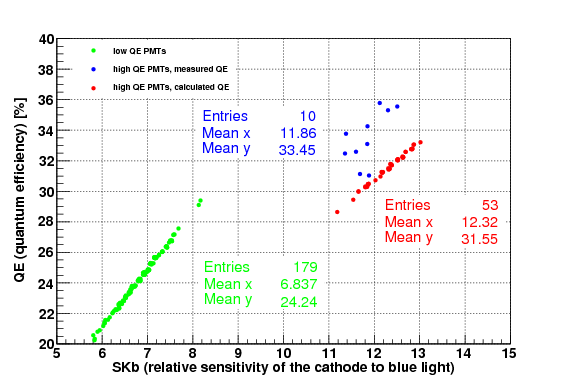
\includegraphics[width=0.475\linewidth]{plots/QE/QEvsSKB_3types.png}
%\label{figQEtypes_1}}
%\subfigure[]{
%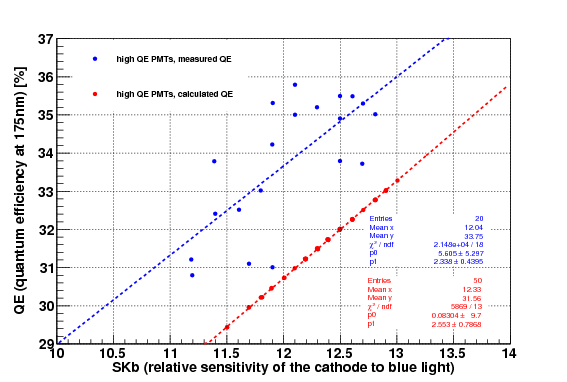
\includegraphics[width=0.475\linewidth]{plots/QE/QEvsSKB_highQE.png}
%\label{figQEtypes_2}}
%\caption{QE and SKb values for the different types of R8520 Hamamatsu PMTs.}
%\label{figQEtypes}
%\end{figure}


\begin{figure}[!h]
\centering
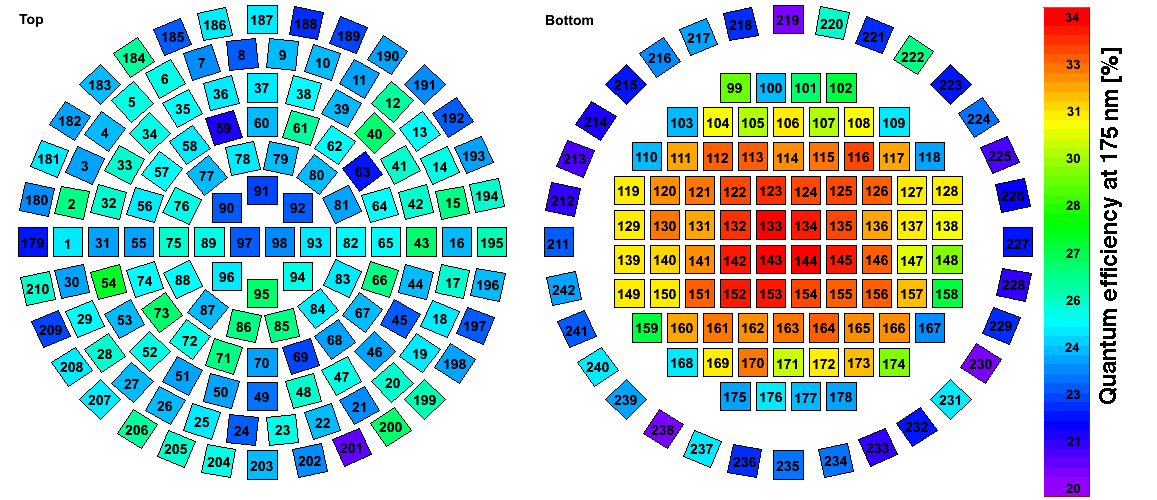
\includegraphics[width=1.0\linewidth]{plots/QE/QEmap.png}
\caption[Quantum efficiency of the XENON100 PMTs]{Quantum efficiency of the XENON100 PMTs. The top array consists of `low QE' PMTs with an average QE of 25\%, and the `high QE' ($\sim$32\%) PMTs are installed on the bottom array.}
\label{figQEmap}
\end{figure}

The calibration curves characterize the average behavior of a PMTs of a given model. The real QE values, which can be obtained in a proper measurement, can differ from one phototube to another  by $\sim$10\%, as can be seen in Fig.~\ref{figPMT_3}. 

Another parameter that affects the overall PMT sensitivity is the photoelectron collection efficiency (CE) at the fist dynode. It defines the probability that photoelectrons emit secondary photons from the first dynode, so that they can be effectively multiplied at the successive dynode stages without deviating from favorable trajectories. The CE depends on the voltage between the photocathode and the first dynode and electric field lines. For the R8520 model used in XENON100 it is typically (80$\pm$10)\%~\cite{PMTmassModel}.

As a consequence of the QE and CE uncertainty, the detection efficiency can differ among the phototubes of the same type by $\sim$10\%. This results in an uncertainty of the amplitude of the signal detected by each PMT, and can affect $XY$ position reconstruction (see Chapter~\ref{chPositionReconstruction}), especially for small signals within the region of interest for the XENON100 experiment. This problem could be eliminated with a measurement of the relative detection efficiency for the XENON100 PMTs.

An {\it in-situ} measurement of the relative detection efficiency for the PMTs within the top array has been performed, using the light calibration setup described in Section~\ref{secGainCalibration}.  For this study, the LED light level has been much higher than required for the gain calibration. The response of each PMT has been fitted with a Gaussian function, and an average light level detected by the PMTs has been determined as $\sim$10~PE. 

In order to interpret the results of the measurement, a Monte Carlo simulation has been performed with GEANT4, using the detailed detector model. The point-like light sources have been defined at the positions of the 4 optical fibers installed in the target volume, and the photons have been generated isotropically. Details on the optical simulation with GEANT4 are given in Sections~\ref{secLCEs1} and \ref{secLCEs2}.

Results of the measurement and the Monte Carlo simulation are presented in Fig.~\ref{figDetectedLight_1} and Fig.~\ref{figDetectedLight_2}, respectively. The PMTs have been grouped according to their position within the different rings of the top array and shown with different colors, see Fig.~\ref{figTopArray_1} and Fig.~\ref{figPMTarrangement}.  For each of these six groups the mean value is calculated, and shown on the plot with solid lines. Both measured and simulated data points are normalized to the mean value of the 1st group (PMTs 1-30), and the measurement is scaled to the curve obtained from the simulation by the mean value of the distribution. The comparison of the measurement and simulation is shown in Fig.~\ref{figQEtopArray_1}. 
The vertical error bars show the standard error of the mean value, and the horizontal bars show a range in radius which is covered by each of the PMT rings. 
%The simulated distribution is fitted with a polynomial function of the 4th order.

\begin{figure}[!h]
\centering
\subfigure[data]{
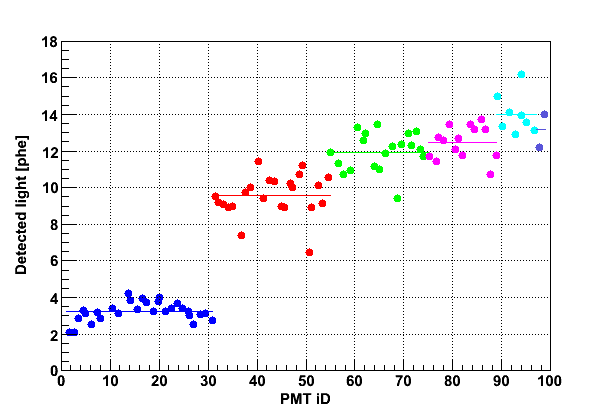
\includegraphics[width=0.475\linewidth]{plots/QE/lightVSpmt_data.png}
\label{figDetectedLight_1}}
\subfigure[MC]{
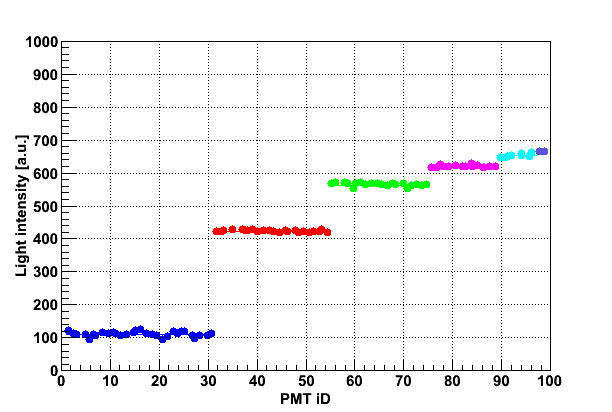
\includegraphics[width=0.475\linewidth]{plots/QE/lightVSpmt_mc.png}
\label{figDetectedLight_2}}
\caption[Light detected by the PMTs of the top array, measured with an LED and simulated with GEANT4]{Light detected by the PMTs of the top array, measured with an LED and simulated with GEANT4. The agreement between Monte Carlo and measured data is remarkable. The 'steps' are due to the difference in geometrical light detection efficiency on the concentric PMTs rings of the top array.}
\label{figDetectedLight}
\end{figure}

In order to calculate the relative PMT detection efficiency, the light intensity on each PMT has been normalized to the average value of the corresponding PMT group (flat lines in Fig.~\ref{figDetectedLight}). The result is shown in Fig.~\ref{figQEtopArray_2}. 
The agreement between the measurement and simulation confirms the validity of this method.  However, the statistical uncertainty of the measurement is on the order of 10\%, which is similar to the spread of the QEs extrapolated using the calibration curves provided by the manufacturer, hence the results of this study have not been used in the subsequent data analysis.

\begin{figure}[!h]
\centering
\subfigure[]{
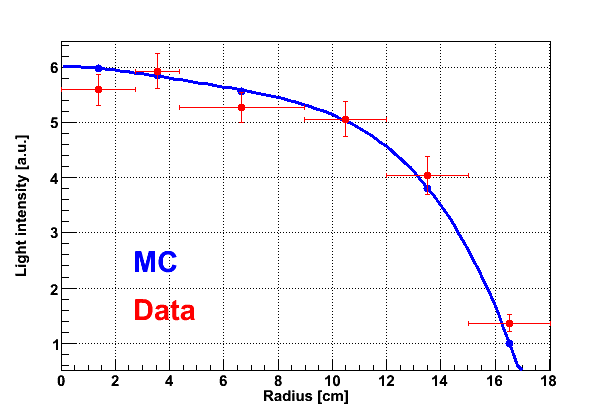
\includegraphics[width=0.475\linewidth]{plots/QE/pol4_dataMC.png}
\label{figQEtopArray_1}}
\subfigure[]{
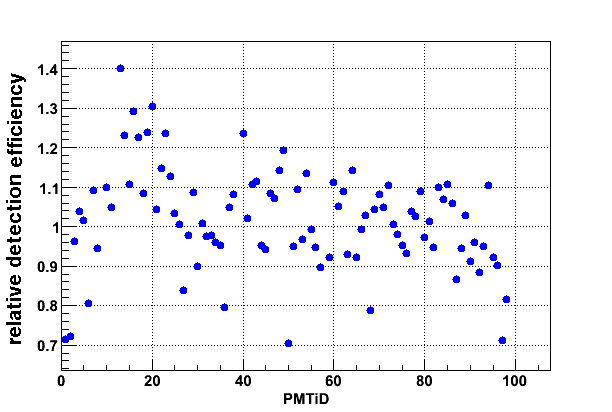
\includegraphics[width=0.475\linewidth]{plots/QE/qeVSpmt_mod.png}
\label{figQEtopArray_2}}
\caption[Normalized light intensity in the measurement and Monte Carlo simulation and measured relative detection efficiency of the top array PMTs]{Normalized light intensity in the measurement and Monte Carlo simulation (a) and measured relative detection efficiency of the top array PMTs (b). The relative light intensity observed for the different PMT rings in the measurement are correctly reproduced by the Monte Carlo simulation. The $\sim$10\% statistical uncertainty of the measurement does not allow to use the measured relative detection efficiency for S2 correction.}
\label{figQEtopArray}
\end{figure}


